
\de{ĐỀ THI HỌC KỲ I NĂM HỌC 2022-2023}{THPT Chuyên Võ Nguyên Giáp - Quảng Bình}
\begin{center}
	\textbf{PHẦN 1 - TRẮC NGHIỆM}
\end{center}
\Opensolutionfile{ans}[ans/ans]
\begin{ex}%[0D1B1-3]%[Dự án đề kiểm tra HK1 NH22-23-Nhật Thiện]%[Chuyên Võ Nguyên Giáp - Quảng Bình]
	Phủ định của mệnh đề \lq\lq Tất cả học sinh lớp $10$ đều thích cầu thủ Lionel Messi\rq\rq là mệnh đề nào?
	\choice
	{\lq\lq Tất cả học sinh lớp $10$ đều không thích cầu thủ Lionel Messi\rq\rq}
	{\True \lq\lq Có học sinh lớp $10$ không thích cầu thủ Lionel Messi\rq\rq}
	{\lq\lq Chỉ có ít học sinh lớp $10$ thích cầu thủ Lionel Messi\rq\rq}
	{\lq\lq Có nhiều học sinh lớp 10 thích cầu thủ Lionel Messi\rq\rq}
\loigiai{
Mệnh đề phủ định của của mệnh đề \lq\lq Tất cả học sinh lớp $10$ đều thích cầu thủ Lionel Messi\rq\rq là \lq\lq Có học sinh lớp $10$ không thích cầu thủ Lionel Messi\rq\rq.
}
\end{ex}
\begin{ex}%[0D1B1-4]%[Dự án đề kiểm tra HK1 NH22-23-Nhật Thiện]%[Chuyên Võ Nguyên Giáp - Quảng Bình]
	Sử dụng thuật ngữ \lq\lq điều kiện đủ\rq\rq để phát biểu định lý \lq\lq Nếu hai tam giác bằng nhau thì chúng có diện tích bằng nhau\rq\rq.
	\choice
	{\True Hai tam giác bằng nhau là điều kiện đủ để hai tam giác đó có diện tích bằng nhau}
	{Hai tam giác có diện tích bằng nhau là điều kiện đủ để hai tam giác đó bằng nhau}
	{Hai tam giác có diện tích bằng nhau là điều kiện cần và đủ để hai tam giác đó bằng nhau}
	{Hai tam giác bằng nhau khi và chỉ khi là tam giác đó có diện tích bằng nhau}
\loigiai{
Hai tam giác bằng nhau là điều kiện đủ để chúng có diện tích bằng nhau.
}
\end{ex}
\begin{ex}%[0D1Y1-1]%[Dự án đề kiểm tra HK1 NH22-23-Nhật Thiện]%[Chuyên Võ Nguyên Giáp - Quảng Bình]
	Trong các khẳng định sau, khẳng định nào \textbf{không phải} là mệnh đề?
	\choice
	{\True Trận chung kết World Cup 2022 thật thú vị!}
	{Trận chung kết World Cup 2022 là trận chung kết thứ tám trong lịch sử World Cup thi đấu ở hiệp phụ}
	{Người cầm còi điều kiển trận chung kết World cup 2022 là Szymon Marciniak, trọng tài người Ba Lan}
	{Argentina vô địch World Cup 2022}
\loigiai{
Khẳng định \lq\lq Trận chung kết World Cup 2022 thật thú vị!\rq\rq không phải là mệnh đề.
}
\end{ex}
\begin{ex}%[0D1Y1-4]%[Dự án đề kiểm tra HK1 NH22-23-Nhật Thiện]%[Chuyên Võ Nguyên Giáp - Quảng Bình]
	Mệnh đều đảo của mệnh đề \lq\lq Với hai số thực $a$, $b$; nếu $a=b$ thì $a^2=b^2$\rq\rq là
	\choice
	{Với hai số thực $a$, $b$ ta có $a^2=b^2$ khi và chỉ khi $a=b$}
	{\True Với hai số thực $a$, $b$; nếu $a^2=b^2$ thì $a=b$}
	{Với hai số thực $a$, $b$ thì $a^2=b^2$ là điều kiện cần để $a=b$}
	{Với hai số thực $a$, $b$ thì $a=b$ là điều kiện đủ để $a^2=b^2$}
\loigiai{
Mệnh đều đảo của mệnh đề \lq\lq Với hai số thực $a$, $b$; nếu $a=b$ thì $a^2=b^2$\rq\rq là \lq\lq Với hai số thực $a$, $b$; nếu $a^2=b^2$ thì $a=b$\rq\rq.
}
\end{ex}
\begin{ex}%[0D1B2-2]%[Dự án đề kiểm tra HK1 NH22-23-Nhật Thiện]%[Chuyên Võ Nguyên Giáp - Quảng Bình]
	Số tập hợp con của tập hợp $A=\{1;2\}$ là
	\choice
	{$1$}
	{$2$}
	{$3$}
	{\True $4$}
\loigiai{
Số tập hợp con của $A$ là $4$.
}
\end{ex}
\begin{ex}%[0D1Y2-2]%[Dự án đề kiểm tra HK1 NH22-23-Nhật Thiện]%[Chuyên Võ Nguyên Giáp - Quảng Bình]
	Cho tập hợp $A$. Trong các mệnh đề sau, mệnh đề nào sai?
	\choice
	{$\emptyset\subset A$}
	{$A\ne \{A\}$}
	{\True $A\in A$}
	{$A\subset A$}
\loigiai{
Mệnh đề $A\in A$ là mệnh đề sai.
}
\end{ex}
\begin{ex}%[0D1B3-5]%[Dự án đề kiểm tra HK1 NH22-23-Nhật Thiện]%[Chuyên Võ Nguyên Giáp - Quảng Bình]
	Cho tập hợp $A=\{x\in \mathbb{R}|2\le x<5\}$. Phần bù của tập hợp $A$ trong $\mathbb{R}$ là
	\choice
	{$[5;+\infty)$}
	{\True $(-\infty;2)\cup [5;+\infty)$}
	{$(-\infty;2)$}
	{$(-\infty;2]\cup (5;+\infty)$}
\loigiai{
Ta có $A=[2;5)$ suy ra phần bù của $A$ trong $\mathbb{R}$ là $(-\infty;2)\cup [5;+\infty)$.
}
\end{ex}
\begin{ex}%[0D1B3-4]%[Dự án đề kiểm tra HK1 NH22-23-Nhật Thiện]%[Chuyên Võ Nguyên Giáp - Quảng Bình]
	Cho tập hợp $A=(-\infty;3]$ và $B=(1;5]$. Khi đó tập hợp $A\cap B$ là
	\choice
	{\True $(1;3]$}
	{$(3;5]$}
	{$(-\infty;5]$}
	{$(-\infty;1)$}
\loigiai{
Ta có $A\cap B=(1;3]$.
}
\end{ex}
\begin{ex}%[0D2Y1-1]%[Dự án đề kiểm tra HK1 NH22-23-Nhật Thiện]%[Chuyên Võ Nguyên Giáp - Quảng Bình]
	Trong các cặp số sau đây, cặp nào \textbf{không} là nghiệm của bất phương trình $x-4y+5\ge 0$?
	\choice
	{$(-5;0)$}
	{\True $(-2;1)$}
	{$(1;-3)$}
	{$(0;0)$}
\loigiai{
Xét cặp số $(-2;1)$, ta có $-2-4\cdot 1+5\ge 0$ là mệnh đề sai. \\
Vậy $(-2;1)$ không là nghiệm của bất phương trình $x-4y+5\ge 0$.
}
\end{ex}
\begin{ex}%[0D2Y2-2]%[Dự án đề kiểm tra HK1 NH22-23-Nhật Thiện]%[Chuyên Võ Nguyên Giáp - Quảng Bình]
	Điểm $O(0;0)$ \textbf{không} thuộc miền nghiệm của hệ bất phương trình nào sau đây?
	\choice
	{\True $\heva{&x+3y<0\\&2x+y+4>0}$}
	{$\heva{&x+3y\ge 0\\&2x+y-4<0}$}
	{$\heva{&x+3y-6<0\\&2x+y+4>0}$}
	{$\heva{&x+3y-6<0\\&2x+y+4\ge 0}$}
\loigiai{
Xét $\heva{&x+3y<0\\&2x+y+4>0}$, với điểm $O(0;0)$ ta thấy
$0+3\cdot 0<0$ là mệnh đề sai.\\
Vậy $O(0;0)$ không thuộc miền nghiệm của hệ bất phương trình trên.
}
\end{ex}
\begin{ex}%[0D2B1-2]%[Dự án đề kiểm tra HK1 NH22-23-Nhật Thiện]%[Chuyên Võ Nguyên Giáp - Quảng Bình]
	\immini{Nửa mặt phẳng phần không bị gạch (kể cả đường thẳng $d$) ở hình bên là miền nghiệm của bất phương trình nào sau đây?
	\choice
	{$3x+y\le 3$}
	{$x+3y\le 3$}
	{\True $3x+y\ge 3$}
	{$x+3y\ge 3$}}{
\begin{tikzpicture}[scale=1, font=\footnotesize, line join=round, line cap=round, >=stealth]
	\begin{scope}[yscale=.8]
		\begin{scope}
			\clip (-2.2,-1.5) rectangle (1.5,3.5);
			\fill[opacity=.2,pattern=north east lines] (-4.2,15.6)--(-4.2,-4.5)--(2.5,-4.5)--cycle;
			\draw (-0.17,3.5)--(1.5,-1.5) node [pos=0.45, above, sloped] {$d$};
		\end{scope}
		\draw[->] (-2.2,0)--(1.5,0) node[below right]{$x$};
		\draw[->] (0,-1.5)--(0,3.5) node[above left]{$y$};
		\draw (0,0) node[below left]{$O$};
		\foreach \x in {1}
		\draw[thin] (\x,1pt)--(\x,-1pt) node [above] {$\x$};
		\foreach \y in {3}
		\draw[thin] (1pt,\y)--(-1pt,\y) node [right] {$\y$};
	\end{scope}
\end{tikzpicture}
}
\loigiai{
Quan sát hình vẽ, đường thẳng $d$ đi qua $(1;0)$ và $(0;3)$ nên có phương trình $y=-3x+3$.\\
Và điểm $O(0;0)$ không thuộc miền nghiệm bất phương trình.\\
Vậy bất phương trình đã cho là $3x+y\ge 3$.
}
\end{ex}
\begin{ex}%[0D2Y2-1]%[Dự án đề kiểm tra HK1 NH22-23-Nhật Thiện]%[Chuyên Võ Nguyên Giáp - Quảng Bình]
	Trong các hệ sau hệ nào \textbf{không phải} là hệ bất phương trình bậc nhất hai ẩn?
	\choice
	{\True $\heva{&x-y<4\\&x^2+2y\le 15}$}
	{$\heva{&x-1>3\\&y+3\le \pi}$}
	{$\heva{&x-2y>4\\&2x+y\le 12\\&y\ge 1}$}
	{$\heva{&x+2y\le 14\\&-3<x\le 5}$}
\loigiai{
Hệ $\heva{&x-y<4\\&x^2+2y\le 15}$ không phải là hệ bất phương trình bậc nhất hai ẩn.
}
\end{ex}
\begin{ex}%[0D2B2-2]
	\immini{Miền trong tam giác $ABC$ kể cả ba cạnh ở hình bên là miền nghiệm của hệ bất phương trình nào trong các hệ sau?
	\choice
	{$\heva{&y\ge 0\\&5x-4y\ge 10\\&5x+4y\le 10}$}
	{$\heva{&x\ge 0\\&4x-5y\le 10\\&5x+4y\le 10}$}
	{\True $\heva{&x\ge 0\\&5x-4y\le 10\\&4x+5y\le 10}$}
	{$\heva{&x>0\\&5x-4y\le 10\\&4x+5y\le 10}$}}{
	\begin{tikzpicture}[scale=1, font=\footnotesize, line join=round, line cap=round, >=stealth]
		\begin{scope}
			\clip (-.5,-3) rectangle (3,2.5);
			\fill[opacity=.2,pattern=north east lines] (0,-3)--(-.5,-3)--(-.5,2.5)--(0,2.5)--cycle;
			\fill[opacity=.2,pattern=north east lines] (-1.5,-4.38)--(5,-4.38)--(5,3.75)--cycle;
			\fill[opacity=.2,pattern=north east lines] (-1.5,3.2)--(7,3.2)--(7,-3.6)--cycle;
			\draw (4,2.5)--(-0.4,-3);
			\draw (-0.62,2.5)--(6.25,-3);
		\end{scope}
		\draw[->] (-.5,0)--(3,0) node[below]{$x$};
		\draw[->] (0,-3)--(0,2.5) node[left]{$y$};
		\draw (0,0) node[below left]{$O$};
		\foreach \x in {1,2}
		\draw[thin] (\x,1pt)--(\x,-1pt) node [below] {$\x$};
		\foreach \y in {-1,-2,1,2}
		\draw[thin] (1pt,\y)--(-1pt,\y) node [left] {$\y$};
		\draw[fill=black] (0,2) circle (1pt) node[right]{$A$} 
		(90/41,10/41) circle (1pt) node [left]{$B$}
		(0,-2.5) circle (1pt) node[right]{$C$} node[left]{$-2,5$}
		(2.5,0) circle (1pt) node[below]{$2,5$}
		;
	\end{tikzpicture}
}
\loigiai{
Quan sát hình vẽ, phương trình đường thẳng chứa các cạnh của tam giác $ABC$ lần lượt là $x=0$; $5x-4y-10=0$ và $4x+5y-10=0$.\\
Và điểm $(1;1)$ thuộc miền nghiệm của hệ bất phương trình.\\
Vậy hệ bất phương trình đã cho là $\heva{&x\ge 0\\&5x-4y\le 10\\&4x+5y\le 10}$.
}
\end{ex}
\begin{ex}%[0H1B1-2]%[Dự án đề kiểm tra HK1 NH22-23-Nhật Thiện]%[Chuyên Võ Nguyên Giáp - Quảng Bình]
	Cho góc $\alpha=xOM$ với điểm $M\left(\dfrac{1}{3};\dfrac{2\sqrt{2}}{3}\right)$ nằm trên nửa đường tròn đơn vị. Giá trị của $\cot \alpha$ là
	\choice
	{\True $\cot \alpha=\dfrac{\sqrt{2}}{4}$}
	{$\cot \alpha=2\sqrt{2}$}
	{$\cot \alpha=\dfrac{1}{3}$}
	{$\cot \alpha=\dfrac{2\sqrt{2}}{3}$}
\loigiai{
Góc $\alpha=xOM$ với điểm $M\left(\dfrac{1}{3};\dfrac{2\sqrt{2}}{3}\right)$ nằm trên nửa đường tròn đơn vị. \\
Khi đó $\cos \alpha=\dfrac{1}{3}$, $\sin \alpha=\dfrac{2\sqrt{2}}{3}$.\\
Vậy $\cot \alpha=\dfrac{\cos \alpha}{\sin \alpha}=\dfrac{1}{2\sqrt{2}}=\dfrac{\sqrt{2}}{4}$.
}
\end{ex}
\begin{ex}%[0H1B1-1]%[Dự án đề kiểm tra HK1 NH22-23-Nhật Thiện]%[Chuyên Võ Nguyên Giáp - Quảng Bình]
	Cho góc $\alpha$ $(90^\circ<\alpha<180^\circ)$. Khẳng định nào sau đây \textbf{đúng}?
	\choice
	{$\cos \alpha>0$}
	{\True $\sin \alpha>0$}
	{$\tan \alpha>0$}
	{$\cot \alpha>0$}
\loigiai{
Góc $90^\circ<\alpha<180^\circ$ suy ra $\sin \alpha>0$.
}
\end{ex}
\begin{ex}%[0H1B1-2]%[Dự án đề kiểm tra HK1 NH22-23-Nhật Thiện]%[Chuyên Võ Nguyên Giáp - Quảng Bình]
	Cho $90^\circ<\alpha<180^\circ$ và thỏa mãn $\sin \alpha=\dfrac{1}{3}$. Giá trị của $\cot \alpha$ bằng
	\choice
	{$-\dfrac{\sqrt{2}}{4}$}
	{$\dfrac{\sqrt{2}}{4}$}
	{$2\sqrt{2}$}
	{\True $-2\sqrt{2}$}
\loigiai{
Ta có $\sin^2\alpha+\cos^2\alpha=1\Rightarrow \cos^2\alpha=1-\sin^2\alpha=\dfrac{8}{9}$.\\
Mà $90^\circ<\alpha<180^\circ$ nên $\cos \alpha<0$ suy ra $\cos \alpha=-\dfrac{2\sqrt{2}}{3}$.\\
Vậy $\cot \alpha=\dfrac{\cos \alpha}{\sin \alpha}=-2\sqrt{2}$.
}
\end{ex}
\begin{ex}%[0H1B2-2]%[Dự án đề kiểm tra HK1 NH22-23-Nhật Thiện]%[Chuyên Võ Nguyên Giáp - Quảng Bình]
	Cho $\triangle ABC$ có các cạnh $BC=a$, $AC=b$, $AB=c$, $R$, $r$ lần lượt là bán kính đường tròn ngoại tiếp, đường tròn nội tiếp $\triangle ABC$, $p$ là nửa chi vi, $S$ là diện tích của tam giác $ABC$. Mệnh đề nào sau đây \textbf{sai}?
	\choice
	{$S=pr$}
	{$S=\dfrac{1}{2}ab\sin C$}
	{\True $S=\dfrac{4R}{abc}$}
	{$S=\sqrt{p(p-a)(p-b)(p-c)}$}
\loigiai{
Diện tích $S$ của tam giác $ABC$ là $S=\dfrac{abc}{4R}$.
}
\end{ex}
\begin{ex}%[0H1B2-1]%[Dự án đề kiểm tra HK1 NH22-23-Nhật Thiện]%[Chuyên Võ Nguyên Giáp - Quảng Bình]
	Tam giác $ABC$ có các góc $\widehat{B}=30^\circ$, $\widehat{C}=45^\circ$ và cạnh $AB=3$. Khi đó cạnh $AC$ bằng
	\choice
	{$\dfrac{3\sqrt{6}}{2}$}
	{\True $\dfrac{3\sqrt{2}}{2}$}
	{$\sqrt{6}$}
	{$\dfrac{2\sqrt{6}}{3}$}
\loigiai{
Theo định lí $\sin$, ta có 
$$\dfrac{AB}{\sin C}=\dfrac{AC}{\sin B}\Rightarrow AC=\dfrac{AB\cdot \sin B}{\sin C}=\dfrac{3\cdot \sin 30^\circ}{\sin 45^\circ}=\dfrac{3\sqrt{2}}{2}.$$
}
\end{ex}
\begin{ex}%[0H1B2-1]%[Dự án đề kiểm tra HK1 NH22-23-Nhật Thiện]%[Chuyên Võ Nguyên Giáp - Quảng Bình]
	Cho tam giác $ABC$ có $BC^2+CA^2-AB^2<0$. Khẳng định nào sau đây đúng?
	\choice
	{\True $\triangle ABC$ tù}
	{$\widehat{A}>90^\circ$}
	{$\triangle ABC$ nhọn}
	{$\triangle ABC$ vuông}
\loigiai{
Theo hệ quả định lí côsin, ta có 
$\cos C=\dfrac{BC^2+CA^2-AB^2}{2BC\cdot CA}<0$.\\
Mà $0^\circ<\widehat{C}<180^\circ$ suy ra $\widehat{C}$ tù.\\
Vậy tam giác $ABC$ là tam giác tù.
}
\end{ex}
\begin{ex}%[0H1B2-2]%[Dự án đề kiểm tra HK1 NH22-23-Nhật Thiện]%[Chuyên Võ Nguyên Giáp - Quảng Bình]
	Cho tam giác $ABC$ có $\widehat{BAC}=150^\circ$, $AC=6$ cm, $S_{\triangle ABC}=6$ cm$^2$. Độ dài cạnh $AB$ bằng
	\choice
	{$4$ cm}
	{$6$ cm}
	{$8$ cm}
	{\True $2$ cm}
\loigiai{
Ta có $S_{\triangle ABC}=\dfrac{1}{2}AB\cdot AC\Rightarrow AB=\dfrac{2S_{\triangle ABC}}{AC}=\dfrac{2\cdot 6}{6}=2$ cm.
}
\end{ex}
\begin{ex}%[0H2B3-2]%[Dự án đề kiểm tra HK1 NH22-23-Nhật Thiện]%[Chuyên Võ Nguyên Giáp - Quảng Bình]
	Cho $G$ là trọng tâm của tam giác $ABC$, $M$ là trung điểm của $BC$. Đẳng thức nào sau đây đúng?
	\choice
	{$\vec{GA}=2\vec{GM}$}
	{\True $\vec{GA}+\vec{GB}+\vec{GC}=\vec{0}$}
	{$\vec{AM}+\vec{BM}+\vec{CM}=3\vec{MG}$}
	{$\vec{GB}+\vec{GC}=\vec{GM}$}
\loigiai{
Ta có $G$ là trọng tâm của tam giác $ABC$ suy ra $\vec{GA}+\vec{GB}+\vec{GC}=\vec{0}$.
}
\end{ex}
\begin{ex}%[0H2B3-1]%[Dự án đề kiểm tra HK1 NH22-23-Nhật Thiện]%[Chuyên Võ Nguyên Giáp - Quảng Bình]
	Cho hình vuông $ABCD$ cạnh $a$. Tính $\left|\vec{AB}+\vec{AC}+\vec{AD}\right|$.
	\choice
	{$3a$}
	{$(2+\sqrt{2})a$}
	{$a\sqrt{2}$}
	{\True $2\sqrt{2}a$}
\loigiai{
Ta có 
$$\left|\vec{AB}+\vec{AC}+\vec{AD}\right|=\left|2\vec{AC}\right|=2AC=2\cdot AB\sqrt{2}=2a\sqrt{2}.$$
}
\end{ex}
\begin{ex}%[0H3Y1-3]%[Dự án đề kiểm tra HK1 NH22-23-Nhật Thiện]%[Chuyên Võ Nguyên Giáp - Quảng Bình]
	Trong hệ trục tọa độ $Oxy$, cho $\vec{v}=3\vec{i}-2\vec{j}$. Tọa độ của $\vec{v}$ là
	\choice
	{$\vec{v}=(3;2)$}
	{\True $\vec{v}=(3;-2)$}
	{$\vec{v}=(2;3)$}
	{$\vec{v}=(-2;3)$}
\loigiai{
Tọa độ của $\vec{v}$ là $\vec{v}=(3;-2)$.
}
\end{ex}
\begin{ex}%[0H3Y1-3]%[Dự án đề kiểm tra HK1 NH22-23-Nhật Thiện]%[Chuyên Võ Nguyên Giáp - Quảng Bình]
	Trong hệ tọa độ $Oxy$, cho $A(5;2)$, $B(10;8)$. Tọa độ của véc-tơ $\vec{AB}$ là
	\choice
	{$\vec{AB}=\left(\dfrac{15}{2};5\right)$}
	{$\vec{AB}=(-5;-6)$}
	{\True $\vec{AB}=(5;6)$}
	{$\vec{AB}=(15;10)$}
\loigiai{
Tọa độ của véc-tơ $\vec{AB}$ là $\vec{AB}=(5;6)$.
}
\end{ex}
\begin{ex}%[0H3B1-3]%[Dự án đề kiểm tra HK1 NH22-23-Nhật Thiện]%[Chuyên Võ Nguyên Giáp - Quảng Bình]
	Trong hệ tọa độ $Oxy$, cho hình bình hành $ABCD$ có $A(0;3)$, $B(2;1)$, $C(-1;0)$. Tọa độ điểm $D$ là
	\choice
	{$D(-3;-2)$}
	{$D(3;2)$}
	{\True $D(-3;2)$}
	{$D(3;-2)$}
\loigiai{
Ta có $ABCD$ là hình bình hành suy ra $\vec{AB}=\vec{DC}\Rightarrow \heva{&x_D=x_A+x_C-x_B\\&y_D=y_A+y_C-y_B}\Leftrightarrow \heva{&x_D=-3\\&y_D=2.}$\\
Vậy $D(-3;2)$.
}
\end{ex}
\begin{ex}%[0H2Y4-1]%[Dự án đề kiểm tra HK1 NH22-23-Nhật Thiện]%[Chuyên Võ Nguyên Giáp - Quảng Bình]
	Cho hai véc-tơ $\vec{a}$ và $\vec{b}$ đều khác $\vec{0}$. Khẳng định nào sau đây đúng?
	\choice
	{$\vec{a}\cdot \vec{b}=\left|\vec{a}\cdot \vec{b}\right|\cdot \cos \left(\vec{a}, \vec{b}\right)$}
	{$\vec{a}\cdot \vec{b}=\left|\vec{a}\right|\cdot \left|\vec{b}\right|\cdot \sin \left(\vec{a},\vec{b}\right)$}
	{$\vec{a}\cdot \vec{b}=\left|\vec{a}\right|\cdot \left|\vec{b}\right|$}
	{\True $\vec{a}\cdot \vec{b}=\left|\vec{a}\right|\cdot \left|\vec{b}\right|\cdot \cos \left(\vec{a},\vec{b}\right)$}
\loigiai{
Hai véc-tơ $\vec{a}$ và $\vec{b}$ đều khác $\vec{0}$, khi đó $\vec{a}\cdot \vec{b}=\left|\vec{a}\right|\cdot \left|\vec{b}\right|\cdot \cos \left(\vec{a},\vec{b}\right)$.
}
\end{ex}
\begin{ex}%[0H3B2-1]%[Dự án đề kiểm tra HK1 NH22-23-Nhật Thiện]%[Chuyên Võ Nguyên Giáp - Quảng Bình]
	Trong mặt phẳng $Oxy$, cho tam giác $ABC$ biết $A(1;3)$, $B(-2;-2)$, $C(3;1)$. Giá trị $\cos \widehat{BAC}$ bằng
	\choice
	{$\cos \widehat{BAC}=-\dfrac{1}{\sqrt{17}}$}
	{\True $\cos \widehat{BAC}=\dfrac{1}{\sqrt{17}}$}
	{$\cos \widehat{BAC}=\dfrac{2}{\sqrt{17}}$}
	{$\cos \widehat{BAC}=-\dfrac{2}{\sqrt{17}}$}
\loigiai{
Ta có $\vec{AB}=(-3;-5)$, $\vec{AC}=(2;-2)$ suy ra $AB=\sqrt{34}$, $AC=2\sqrt{2}$. Khi đó
$$\cos \widehat{BAC}=\cos \left(\vec{AB},\vec{AC}\right)=\dfrac{\vec{AB}\cdot \vec{AC}}{AB\cdot AC}=\dfrac{1}{\sqrt{17}}.$$
}
\end{ex}
\begin{ex}%[0X1Y1-3]%[Dự án đề kiểm tra HK1 NH22-23-Nhật Thiện]%[Chuyên Võ Nguyên Giáp - Quảng Bình]
	Viết số quy tròn của số gần đúng $a$ biết $\overline{a}=18658\pm 25$.
	\choice
	{$19000$}
	{$18660$}
	{$18600$}
	{\True $18700$}
\loigiai{
Số quy tròn của số gần đúng $a$ là $18700$.
}
\end{ex}
\begin{ex}%[0X1Y1-1]%[Dự án đề kiểm tra HK1 NH22-23-Nhật Thiện]%[Chuyên Võ Nguyên Giáp - Quảng Bình]
	Đo chiều dài của một cây thước, ta được kết quả $\overline{a}=50\pm0{,}2$ cm. Khi đó sai số tuyệt đối của phép đo được ước lượng là 
	\choice
	{\True $\Delta_{50}=0{,}2$ cm}
	{$\Delta_{50}\le 0{,}2$ cm}
	{$\Delta_{50}\le -0{,}2$ cm}
	{$\Delta_{50}=-0{,}2$ cm}
\loigiai{
Sai số tuyệt đối của phép đo được ước lượng là $\Delta_{50}=0{,}2$ cm.
}
\end{ex}
\begin{ex}%[0X1B3-2]%[Dự án đề kiểm tra HK1 NH22-23-Nhật Thiện]%[Chuyên Võ Nguyên Giáp - Quảng Bình]
	Đo chỉ số IQ của một nhóm $11$ học sinh được kết quả như sau
	\begin{center}
		\begin{tabular}{ccccccccccc}
			$60$& $72$ & $63$ & $83$ & $68$ & $90$ & $74$ & $86$ & $74$ & $80$ & $82$
		\end{tabular}
	\end{center}
	Số trung vị của mẫu số liệu trên là
	\choice
	{$73$}
	{\True $74$}
	{$90$}
	{$68$}
\loigiai{
Mẫu số liệu được xếp lại theo thứ tự không giảm như sau
\begin{center}
	\begin{tabular}{ccccccccccc}
		$60$ & $63$  & $68$ & $72$ & $74$ & $74$ & $80$ & $82$ & $83$ & $86$ & $90$
	\end{tabular}
\end{center}
Mẫu trên có trung vị là $M_{\mathrm{e}}=74$.
}
\end{ex}
\begin{ex}%[0X1B3-3]%[Dự án đề kiểm tra HK1 NH22-23-Nhật Thiện]%[Chuyên Võ Nguyên Giáp - Quảng Bình]
	Mẫu số liệu về điểm kiểm tra $9$ môn của một học sinh như sau
	\begin{center}
		\begin{tabular}{ccccccccc}
			$6{,}5$ & $8$ & $9$ & $8{,}5$ & $7$ & $7{,}5$ & $6$ & $7{,}25$ & $9{,}5$
		\end{tabular}
	\end{center}
	Tứ phân vị của mẫu số liệu trên là
	\choice
	{$Q_1=6{,}75$, $Q_2=7$, $Q_3=7{,}5$}
	{\True $Q_1=6{,}75$, $Q_2=7{,}5$, $Q_3=8{,}75$}
	{$Q_1=7{,}5$, $Q_2=7$, $Q_3=8{,}75$}
	{$Q_1=8{,}5$, $Q_2=7$, $Q_3=6{,}625$}
\loigiai{
Mẫu số liệu được xếp lại theo thứ tự không giảm như sau
\begin{center}
\begin{tabular}{ccccccccc}
	$6$ & $6{,}5$ & $7$ & $7{,}25$ & $7{,}5$ & $8$ & $8{,}5$ & $9$ & $9{,}5$
\end{tabular}
\end{center}
Giá trị của tứ phân vị thứ hai là $Q_2=M_{\mathrm{e}}=7{,}5$.\\
Giá trị của tứ phân vị thứ nhất là $Q_1=\dfrac{6{,}5+7}{2}=6{,}75$.\\
Giá trị của tứ phân vị thứ ba là $Q_3=\dfrac{8{,}5+9}{2}=8{,}75$.
}
\end{ex}
\begin{ex}%[0X1Y3-5]%[Dự án đề kiểm tra HK1 NH22-23-Nhật Thiện]%[Chuyên Võ Nguyên Giáp - Quảng Bình]
	Giá trị xuất hiện với tần số lớn nhất của mẫu số liệu được gọi là
	\choice
	{Số trung bình}
	{Trung vị}
	{Tần suất}
	{\True Mốt}
\loigiai{
Giá trị xuất hiện với tần số lớn nhất của mẫu số liệu được gọi là Mốt.
}
\end{ex}
\begin{ex}%[0X1B4-1]%[Dự án đề kiểm tra HK1 NH22-23-Nhật Thiện]%[Chuyên Võ Nguyên Giáp - Quảng Bình]
	Đểm kiểm tra giữa kỳ 1 môn Toán của $10$ bạn học sinh như sau
	\begin{center}
		\begin{tabular}{cccccccccc}
			$6{,}5$ & $8$  & $9$ & $8{,}5$ & $7$ & $9{,}8$ & $7{,}5$ & $6$ & $7{,}25$ & $9{,}5$
		\end{tabular}
	\end{center}
	Khoảng biến thiên của mẫu số liệu trên là
	\choice
	{$3{,}0$}
	{$3{,}5$}
	{\True $3{,}8$}
	{$3{,}3$}
\loigiai{
Mẫu số liệu được xếp lại theo thứ tự không giảm như sau
\begin{center}
	\begin{tabular}{cccccccccc}
		$6$ & $6{,}5$  & $7$ & $7{,}25$ & $7{,}5$ & $8$ & $8{,}5$ & $9$ & $9{,}5$ & $9{,}8$
	\end{tabular}
\end{center}
Khoảng biến thiên của mẫu số liệu trên là $9{,}8-6=3{,}8$.
}
\end{ex}
\begin{ex}%[0X1Y4-4]%[Dự án đề kiểm tra HK1 NH22-23-Nhật Thiện]%[Chuyên Võ Nguyên Giáp - Quảng Bình]
	Số đặc trưng nào trong các số sau đây đo độ phân tán của mẫu số liệu?
	\choice
	{Số trung bình}
	{Mốt}
	{Trung vị}
	{\True Độ lệch chuẩn}
\loigiai{
Độ lệch chuẩn đo độ phân tán của mẫu số liệu.
}
\end{ex}
\begin{ex}%[0X1B4-2]%[Dự án đề kiểm tra HK1 NH22-23-Nhật Thiện]%[Chuyên Võ Nguyên Giáp - Quảng Bình]
	Cho mẫu số liệu 
	\begin{center}
		\begin{tabular}{cccccccccccc}
			$12$ & $3$ & $6$ & $15$ &$27$ &$33$ & $31$ &$18$ &$29$ &$54$ &$1$ &$8$
		\end{tabular}
	\end{center}
Số giá trị bất thường trong mẫu số liệu trên là
\choice
{\True $0$}
{$1$}
{$2$}
{$3$}
\loigiai{
Mẫu số liệu được xếp lại theo thứ tự không giảm như sau
\begin{center}
	\begin{tabular}{cccccccccccc}
	$1$	&$3$ & $6$ & $8$ & $12$ & $15$ &$18$ & $27$ &$29$ &$31$ &$33$  &$54$
	\end{tabular}
\end{center}
Giá trị của tứ phân vị thứ hai là $Q_2=\dfrac{15+18}{2}=16{,}5$.\\
Giá trị của tứ phân vị thứ nhất là $Q_1=\dfrac{6+8}{2}=7$.\\
Giá trị của tứ phân vị thứ ba là $Q_3=\dfrac{29+31}{2}=30$.\\
Khoảng tứ phân vị $\Delta_Q=Q_3-Q_1=23$.\\
Giá trị bất thường của mẫu số liệu thỏa $\hoac{&x>Q_3+1{,}5\Delta_Q\\&x<Q_1-1{,}5\Delta_Q}\Leftrightarrow \hoac{&x>30+1{,}5\cdot 23\\&x<7-1{,}5\cdot 23}\Leftrightarrow \hoac{&x>64{,}5\\&x<-27{,}5.}$\\
Quan sát mẫu số liệu nhận thấy không có giá trị bất thường.
}
\end{ex}

\Closesolutionfile{ans}
%\begin{center}
%	\textbf{ĐÁP ÁN}
%	\inputansbox{10}{ans/ans}	
%\end{center}


\begin{center}
	\textbf{PHẦN 2 - TỰ LUẬN}
\end{center}


\begin{bt}%[0T2B2-3]%[Dự án đề kiểm tra HKI NH22-23- Lê Hùng Thắng]%[Chuyên Võ Nguyên Giáp - QB]
Cho hệ bất phương trình $ \left\{\begin{aligned}
	&x+y \leq 10\\
	&x+4 y \leq 25\\
	&x \geq 0\\
	&y \geq 0
\end{aligned}\right. (I)$ và biểu thức $F(x;y)=30 x+40 y$ xác định trên miền nghiệm của hệ bất phương trình $(I)$. Hãy biểu diễn miền nghiệm của hệ bất phương trình $(I)$ trên mặt phẳng toạ độ và tìm giá trị lớn nhất của $F(x;y)$.
	\loigiai{
\immini{
$\bullet$ Trên mặt phẳng $Oxy$, vẽ các đường thẳng $x+y = 10$ và
$x+4 y = 25$.\\
Xét miền nghiệm của từng bất phương trình suy ra miền nghiệm của hệ bất phương trình $(I)$ là phần mặt phẳng giới hạn bởi tứ giác $OABC$ kể cả các cạnh của tứ giác.\\
Với $O(0;0)$, $A(10;0)$, $B(5;5)$, $C(0;6{,}25)$.\\
$\bullet$ Xét giá trị của $F(x;y)$ tại các đỉnh $O,A,B,C$ ta có\\
$F(0;0)=0$, $F(10;0)=300$, $F(5;5)=350$, $F(0;6{,}25)=250$.\\
Vậy giá trị lớn nhất của $F(x;y)$ là $F(5;5)=350$.
}
{\begin{tikzpicture}[scale=0.3,>=stealth, font=\footnotesize, line join=round, line cap=round]
	\def\xmin{-2} \def\xmax{12}
	\def\ymin{-2} \def\ymax{12}	
	\def\hsa(#1){10-(#1)}
	\def\hsb(#1){6.25-0.25*(#1)}
	\path (\xmin,\ymax) coordinate (A)
	 (\xmin,\ymin) coordinate (B)
	 (\xmax,\ymin) coordinate (C)
	 (\xmax,\ymax) coordinate (D);
	\draw[color=gray!30,dashed] (\xmin,\ymin) grid (\xmax,\ymax);
	\draw[->] (\xmin,0)--(\xmax,0) node [below]{$x$};
	\draw[->] (0,\ymin)--(0,\ymax) node [right]{$y$};
	\node at (0,0) [below left]{$O$};
	\clip (\xmin+0.1,\ymin+0.1) rectangle (\xmax-0.1,\ymax-0.1);
	\draw[smooth,samples=200,domain=\xmin:\xmax] plot(\x,{\hsa(\x)});
	\draw[smooth,samples=200,domain=\xmin:\xmax] plot(\x,{\hsb(\x)});
	\fill[pattern=north east lines,opacity=0.5] plot[domain=\xmin:\xmax](\x,{\hsa(\x)})--(D)--cycle;
	\fill[pattern=north east lines,opacity=0.5] plot[domain=\xmin:\xmax](\x,{\hsb(\x)})--(D)--(A)--cycle;
	\fill[pattern=north east lines,opacity=0.5] plot[domain=\xmin:\xmax](A)--(B)--(C)--(\xmax,0)--(0,0)--(0,\ymax)--cycle;
%	\draw[dotted] (1,0)|-(0,2);
	\fill (10,0) circle (2pt) node [below] {$A$}
	(5,5) circle (2pt) node [below left] {$B$}
	(0,6.25) circle (2pt) node [below right] {$C$};
	\end{tikzpicture}
}
	}
\end{bt}

\begin{bt}%[0T9K1-3]%[0T9B1-5]%[Dự án đề kiểm tra HKI NH22-23- Lê Hùng Thắng]%[Chuyên Võ Nguyên Giáp - QB]
Trong mặt phẳng tọa độ $Oxy$, cho ba điểm $A(1;-3), B(3;5), C(2;2)$.
\begin{listEX}[1]
	\item Chứng minh rằng $A, B, C$ là ba đỉnh của một tam giác.
	\item Gọi $H$ là trực tâm của tam giác $A B C$, tìm tọa độ điểm $H$.
\end{listEX}
	\loigiai{
\begin{listEX}[1]
	\item Ta có $\overrightarrow{AB}=(2;8)$, $\overrightarrow{AC}=(1;5)$.\\
	Vì $2\cdot 5 \ne 8\cdot 1$ nên $\overrightarrow{AB}$ và $\overrightarrow{AC}$ không cùng phương.\\
	Vậy $A, B, C$ là ba đỉnh của một tam giác.
	\item Gọi $H(x;y)$ là trực tâm của tam giác $ABC$.\\
	Ta có $\overrightarrow{AH}=(x-1;y+3)$, $\overrightarrow{BC}=(-1;-3)$, $\overrightarrow{BH}=(x-3;y-5)$, $\overrightarrow{AC}=(1;5)$.\\
	$H$ là trực tâm của tam giác $A B C$ khi $\heva{&\overrightarrow{AH}\cdot \overrightarrow{BC}=0\\&\overrightarrow{BH}\cdot \overrightarrow{AC}=0}$\\
	$\Leftrightarrow \left\{\begin{aligned}
	&(x-1)\cdot (-1)+(y+3)\cdot (-3)=0\\
	&(x-3)\cdot 1 +(y-5)\cdot 5=0\\
	\end{aligned}\right. \Leftrightarrow \left\{\begin{aligned}
	&x+3y=-8\\	&x+5y=28\\
\end{aligned}\right. \Leftrightarrow \left\{\begin{aligned}
&x=-56\\ &y=16.\end{aligned}\right.$\\
Vậy $H(-56;16)$.
\end{listEX}
	}
\end{bt}

\begin{bt}%[0T1K3-3]%[Dự án đề kiểm tra HKI NH22-23- Lê Hùng Thắng]%[Chuyên Võ Nguyên Giáp - QB]
Lớp $10$ A có $40$ học sinh, trong đó có $18$ học sinh thích học môn Văn, $20$ học sinh thích học môn Toán, $22$ học sinh thích học môn Tiếng Anh, $5$ học sinh thích học cả ba môn Toán, Văn, Tiếng Anh; $6$ học sinh không thích học môn nào trong ba môn trên. Hỏi có bao nhiêu học sinh thích học đúng một môn trong ba môn Toán, Văn, Tiếng Anh?	
	\loigiai{
\immini{
Gọi $x,y,z$ lần lượt là số học sinh chỉ thích đúng một môn trong ba môn Văn, Toán, Anh.\\
Xét biểu đồ Ven như hình vẽ với
$a,b,c$ lần lượt là số học sinh thích đúng hai môn Văn-Toán, Toán-Anh, Anh-Văn.\\
Theo đề bài ta có\\
$\heva{&x+y+z+a+b+c+5=34\\&x=13-(a+c)\\&y=15-(a+b)\\&z=17-(b+c)}$
}
{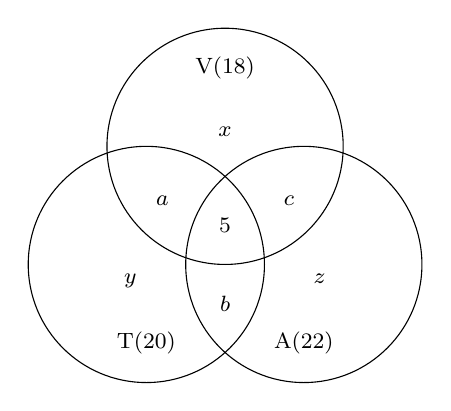
\begin{tikzpicture}[scale=1,>=stealth, font=\footnotesize, line join=round, line cap=round]
%	\draw[dotted] (-2,-2) grid (2,2);
	\draw (0,1.5)circle(1.5);
	\draw(1,0)circle(1.5);
	\draw (-1,0)circle(1.5);
	\draw (0,2.5) node {V($18$)} (0,1.5) node [above] {$x$}
	(-1,-1) node {T($20$)} (-1,0) node [below left]{$y$}
	(1,-1) node {A($22$)} (1,0) node [below right] {$z$}
	(0,0.5) node {$5$}
	(-1,1) node [below right]{$a$} 
	(0,-0.5)  node {$b$} 
	(1,1) node [below left] {$c$};
	\end{tikzpicture}
}
\noindent 
$\Rightarrow \heva{&x+y+z+a+b+c=29\\&x+y+z=45-2(a+b+c)} \Leftrightarrow \heva{&x+y+z=13\\&a+b+c=16.}$\\
Vậy số học sinh thích đúng một môn học là $x+y+z=13$ (học sinh).
}
\end{bt}

\begin{bt}%[0T4G2-2]%[Dự án đề kiểm tra HKI NH22-23- Lê Hùng Thắng]%[Chuyên Võ Nguyên Giáp - QB]
Cho điểm $D$ nằm trong tam giác $ABC$ sao cho $\widehat{DAB}=\widehat{DBC}= \widehat{DCA}=\alpha$. Chứng minh
$$\sin ^3 \alpha=\sin (A-\alpha) \cdot \sin (B-\alpha) \cdot \sin (C-\alpha).$$	
	\loigiai{
\immini{
$\bullet$ Xét tam giác $ABD$ ta có $\dfrac{DB}{\sin \alpha}=\dfrac{A D}{\sin(B-\alpha)}$.\\
$\bullet$ Xét tam giác $BCD$ ta có $\dfrac{CD}{\sin \alpha}=\dfrac{BD}{\sin(C-\alpha)}$.\\
$\bullet$ Xét tam giác $ACD$ ta có $\dfrac{AD}{\sin \alpha}=\dfrac{CD}{\sin(A-\alpha)}$.\\
Từ đó ta có 
$\dfrac{AD \cdot BD \cdot CD}{\sin^3 \alpha} =\dfrac{AD \cdot BD \cdot CD}{\sin(A-\alpha)\cdot \sin(B-\alpha)\cdot\sin(C-\alpha)}$.\\
Vậy $\sin^3 \alpha=\sin(A-\alpha)\cdot \sin(B-\alpha) \cdot \sin(C-\alpha)$.
}
{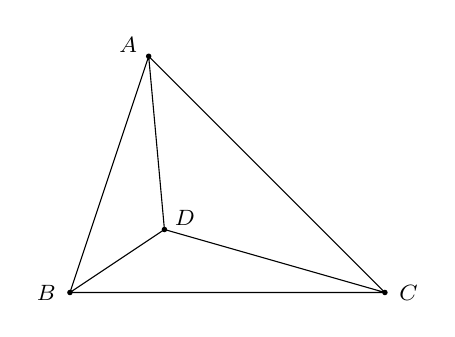
\begin{tikzpicture}[scale=1,>=stealth, font=\footnotesize, line join=round, line cap=round]
	\path (1,3) coordinate (A) 
	(0,0) coordinate (B) 
	(4,0) coordinate (C)
	(1.2,0.8) coordinate (D);
	\draw (A)--(B)--(C)--(A)--(D)--(B) (C)--(D);
	\tkzMarkAngles[size=0.7cm](B,A,D)
	\tkzMarkAngles[size=0.7cm](C,B,D)
	\tkzMarkAngles[size=0.7cm](A,C,D)
	\foreach \d/\g in {A/150,B/180,C/0,D/30} \fill (\d) circle (1pt)++(\g:3mm) node {$\d$};
	\end{tikzpicture}
}
	}
\end{bt}

